\documentclass[11pt]{article}
\usepackage{amsmath, amssymb, amsthm}
\usepackage[margin=1in]{geometry}
\usepackage{float}
\usepackage{graphicx}
\usepackage{subcaption}
\usepackage{booktabs}
\usepackage{enumitem}
\usepackage{pdflscape}
\usepackage{hyperref}
\usepackage[capitalise]{cleveref}
\usepackage{tikz}
\usetikzlibrary{shapes.geometric, arrows.meta, positioning, calc}

% Let two figure floats share a page instead of each claiming one.
\renewcommand{\topfraction}{0.92}
\renewcommand{\bottomfraction}{0.7}
\renewcommand{\textfraction}{0.07}
\renewcommand{\floatpagefraction}{0.8}
\setlength{\floatsep}{10pt plus 2pt minus 2pt}
\setlength{\textfloatsep}{12pt plus 2pt minus 3pt}

\newtheorem{theorem}{Theorem}
\newtheorem{lemma}{Lemma}
\newtheorem{assumption}{Assumption}
\newtheorem{proposition}{Proposition}
\newtheorem{corollary}{Corollary}
\newtheorem{remark}{Remark}

\begin{document}

\begin{abstract}
\begin{enumerate}[label=\arabic*., leftmargin=*, itemsep=2pt, topsep=2pt]
\item The distance matrix $\mathcal{D}$ has a graph form: there is a weighted graph $G_D$
on the $m$ leaves whose effective resistances are the entries of $\mathcal{D}$, and its
Laplacian $L_D$ satisfies $\mathcal{B} := H\mathcal{D}H = -2L_D^{+}$.
\item The vector the algorithm reads, the largest-magnitude eigenvector $u^{(1)}$ of
$\mathcal{B}$, is the Fiedler vector of $L_D$, so its signs cut the leaves along a single
edge of the tree.
\item Stating a recovery guarantee needs two numbers of that vector and that spectrum: the
margin $\delta_* = \min_i |u^{(1)}_i|$ and the gap
$\Delta\lambda = |\lambda_1(\mathcal{B})| - |\lambda_2(\mathcal{B})|$.
\item Observing each distance with probability $p$ and bounding the entrywise eigenvector
error recovers the split exactly at
$p = \Theta\!\left(\frac{d_{\max}^2}{\Delta\lambda^2 \delta_*^2} \log m\right)$.
\begin{enumerate}[label*=\arabic*., leftmargin=*, itemsep=2pt, topsep=2pt]
\item This assumes $u^{(1)}$ is delocalized: $\delta_* \ge c_\delta/\sqrt{m}$ and
$\|u^{(1)}\|_\infty \le C_\delta/\sqrt{m}$.
\item Putting $\Delta\lambda \asymp m$ and $\delta_* \asymp 1/\sqrt{m}$ into that rate
gives $p \gtrsim \log m / m$.
\end{enumerate}
\item What is open is how to read $\Delta\lambda$ and $\delta_*$ off a tree.
\begin{enumerate}[label*=\arabic*., leftmargin=*, itemsep=2pt, topsep=2pt]
\item One way in is to relate $\mathcal{D}$ to the similarity matrix $S = e^{-\mathcal{D}}$,
so that what is known about $L_S$ carries over.
\item The other is to measure both numbers on simulated trees.
\end{enumerate}
\end{enumerate}
\end{abstract}

\newpage


\section{The Distance Matrix and Its Leading Vector}
\label{sec:target}

Two results from the literature carry the argument: the Schur complement results of Stone and Griffing \cite{stone2009fiedler}, which say what the vector looks like on a tree, and the leave-one-out bound of Abbe et al.\ \cite{abbe2020entrywise}, which says how far sampling can move it.

Let $T$ be a weighted tree with $m$ leaves, and let $\mathcal{D}$ be the additive path-distance matrix between the leaves. We apply double centering with the orthogonal projector $H = I - \frac{1}{m}\mathbf{1}\mathbf{1}^\top$ to form the distance operator:
\begin{equation}
\mathcal{B} := H \mathcal{D} H
\end{equation}
The recovery algorithm classifies leaves by the sign pattern of $u^{(1)}$, the unit eigenvector of $\mathcal{B}$ belonging to its largest-magnitude eigenvalue.

\paragraph{Notation.} Two weighted graphs on the $m$ leaves appear throughout, and neither
of their Laplacians is $\mathcal{B}$:
\begin{itemize}
\item $G_S$, with edge weights $S_{ij} = e^{-\mathcal{D}_{ij}}$, and its Laplacian
$L_S = \mathrm{Deg}(S) - S$; this is the operator the similarity route uses.
\item $G_D$, the graph on the leaves whose effective resistances are the distances
$\mathcal{D}_{ij}$, and its Laplacian $L_D$; \Cref{prop:identification} builds it from the
tree and shows $\mathcal{B} = -2L_D^{+}$, so $\mathcal{B}$ is the pseudoinverse of $L_D$ up
to a factor, not $L_D$ itself.
\end{itemize}
$L_T$ denotes the Laplacian of the tree $T$ itself, on all of its vertices, and
$\mathrm{Deg}(W) = \mathrm{diag}(W\mathbf{1})$ for any $W$.

Give each branch $e$ of $T$ its length $\ell_e > 0$ and read $T$ as an electrical network
in which branch $e$ carries conductance $1/\ell_e$. Let $L_T$ be the Laplacian of that
weighted tree, let $R \subset V$ be its internal vertices, and let
\begin{equation}
\label{eq:schur}
L_D \;:=\; L_T \,/\, (L_T)_{RR}
\end{equation}
be the Schur complement of $L_T$ onto the $m$ leaves, taken with respect to its block
$(L_T)_{RR}$ on the internal vertices. With those conductances the effective
resistance between two vertices of a tree is the sum of the branch lengths along the path
joining them \cite{klein1993resistance}, which is exactly $\mathcal{D}_{ij}$.

\begin{proposition}[Identification]
\label{prop:identification}
\leavevmode
\begin{enumerate}
\item[(i)] $L_D$ is the Laplacian of a connected weighted graph $G_D$ on the leaves, and it
carries the same effective resistances as $T$:
$\mathcal{D}_{ij} = (L_D^{+})_{ii} + (L_D^{+})_{jj} - 2 (L_D^{+})_{ij}$.
\item[(ii)] $\mathcal{B} = H\mathcal{D}H = -2L_D^{+}$. In particular $\mathcal{B}$ is negative
semi-definite, which is why its largest-magnitude eigenvalue is its most negative one.
\item[(iii)] If the smallest positive eigenvalue of $L_D$ is simple --- equivalently, if the
gap $\Delta\lambda$ of \Cref{thm:recovery} is positive --- then $u^{(1)}$ is the Fiedler
vector of $G_D$, up to sign.
\end{enumerate}
\end{proposition}

\begin{proof}
(i) The Schur complement of a Laplacian with respect to a set of vertices is again a
Laplacian, of the Kron-reduced graph, and Kron reduction leaves the effective resistances
between the retained vertices unchanged \cite{dorfler2013kron}; connectedness passes from
$T$ to $G_D$. The stated identity is then the standard expression of effective resistance
through the Laplacian pseudoinverse \cite{klein1993resistance}, applied to $G_D$.

(ii) Write $\pi = \mathrm{diag}(L_D^{+})$, so that (i) reads
$\mathcal{D} = \pi \mathbf{1}^\top + \mathbf{1}\pi^\top - 2L_D^{+}$. Since $H\mathbf{1} = 0$,
both rank-one terms drop out under double centering and
$H \mathcal{D} H = -2\, H L_D^{+} H$. The graph $G_D$ is connected, so
$L_D^{+}\mathbf{1} = 0$ and $HL_D^{+}H = L_D^{+}$. Hence $\mathcal{B} = -2L_D^{+}$, and
$L_D^{+} \succeq 0$ gives
$\mathcal{B} \preceq 0$.

(iii) $L_D$ and $L_D^{+}$ share their eigenvectors, an eigenvalue $\lambda > 0$ of $L_D$
becoming $1/\lambda$ of $L_D^{+}$ and the kernel staying the kernel. So the eigenvector of
$L_D$ for its smallest positive eigenvalue is the eigenvector of $L_D^{+}$ for its largest, and by (ii) the
eigenvector of $\mathcal{B}$ for its most negative eigenvalue, which is the largest in
magnitude. That is $u^{(1)}$, and simplicity fixes it up to sign.
\end{proof}

This correspondence between numerical taxonomy and phylogenetics is set out in
\cite{griffing2012}. With it, statements about Fiedler vectors of trees are statements
about $u^{(1)}$.

\begin{lemma}[Target Geometry, {\cite[Theorem 3.3]{stone2009fiedler}}]
\label{lem:target}
The signs of $u^{(1)}$ cut the leaves of $T$ along a single edge: there is one edge $e$ of
$T$ whose removal puts $\{i : u^{(1)}_i > 0\}$ and $\{i : u^{(1)}_i \le 0\}$ in the two
different components.
\end{lemma}

\begin{proof}
Theorem 3.3 of \cite{stone2009fiedler} is stated for a connected weighted graph, for the
Schur complement of its Laplacian with respect to the points of articulation, and for a
Fiedler vector $Y$ of that Schur complement. Here the graph is $T$, its points of
articulation are the internal vertices $R$, the Schur complement is $L_D$ of
\eqref{eq:schur}, and $Y = u^{(1)}$ by \Cref{prop:identification}(iii). The theorem then
supplies a subset $S \subseteq R$ such that $V_+ \cup S$ and $V_- \cup (R-S)$ both induce
connected subgraphs of $T$, where $V_+ = \{i : u^{(1)}_i > 0\}$ and $V_-$ is its
complement among the leaves. Two complementary vertex sets of a tree that are each
connected are joined by exactly one edge, and that edge is $e$.
\end{proof}

The theorem puts a leaf with $u^{(1)}_i = 0$ on the non-positive side, so it gives the
split without claiming that any entry is nonzero. The margin
$\delta_* := \min_i |u^{(1)}_i|$ is a separate quantity, which we assume. For a tree that
is not symmetric $u^{(1)}$ is not piecewise constant, and how far it is from constant
enters only through $\delta_*$.

\begin{assumption}[Delocalization]
\label{as:deloc}
There are constants $c_\delta, C_\delta > 0$ with
$\delta_* \ge c_\delta / \sqrt{m}$ and $\|u^{(1)}\|_\infty \le C_\delta / \sqrt{m}$.
\end{assumption}
The lower half of \Cref{as:deloc} is the one \Cref{lem:target} leaves open, and everything
below uses it wherever $\delta_*$ appears; \Cref{tab:tree-kinds} in Appendix~\ref{app:answer}
reports what it costs on each kind of tree.

Reading \Cref{prop:identification} eigenvalue by eigenvalue says what those two numbers
are.

\begin{corollary}[The two numbers are Fiedler data of $G_D$]
\label{cor:two-numbers}
Let $0 < \mu_1 \le \mu_2 \le \dots \le \mu_{m-1}$ be the positive eigenvalues of $L_D$ and
let $y$ be the Fiedler vector of $G_D$. Then
\begin{equation}
\label{eq:transfer}
|\lambda_1(\mathcal{B})| = \frac{2}{\mu_1}, \qquad
|\lambda_2(\mathcal{B})| = \frac{2}{\mu_2}, \qquad
\Delta\lambda = 2\,\frac{\mu_2 - \mu_1}{\mu_1 \mu_2}, \qquad
\frac{\Delta\lambda}{|\lambda_1(\mathcal{B})|} = 1 - \frac{\mu_1}{\mu_2},
\end{equation}
and $\delta_* = \min_i |y_i|$.
\end{corollary}

\begin{proof}
$\mathcal{B} = -2L_D^{+}$ by \Cref{prop:identification}(ii), and $L_D^{+}$ has eigenvalues
$1/\mu_k$ on the orthogonal complement of $\mathbf{1}$, so the $k$-th largest magnitude
eigenvalue of $\mathcal{B}$ is $2/\mu_k$. The rest is arithmetic, and the last claim is
\Cref{prop:identification}(iii).
\end{proof}

So the rate depends on three properties of one weighted graph on the leaves: its algebraic
connectivity $\mu_1$, the ratio $\mu_1/\mu_2$ to the next eigenvalue, and the smallest
entry of its Fiedler vector. A relative gap of $0.60$ measured on Kingman trees says
$\mu_1/\mu_2 = 0.40$ there.

For a single point of articulation $r$, Stone and Griffing bound the algebraic connectivity of the reduced graph between the two largest
Perron values of the branches hanging at $r$: $\nu_1 < \mu^{-1} < \nu_0$
\cite[Corollary 2.1]{stone2009fiedler}, where $\nu_i = \rho(L_{C_i}^{-1})$ is taken over
the connected components $C_i$ at $r$. Through \eqref{eq:transfer} that reads
$2\nu_1 < |\lambda_1(\mathcal{B})| < 2\nu_0$, a two-sided bound on the leading eigenvalue
in terms of the branches themselves. Extending it to the full internal set $R$, and adding
the companion statement for $\mu_1/\mu_2$ and for $\min_i |y_i|$, is exactly the open
question of \Cref{sec:open}.

\section{Exact Recovery from Sampled Distances}

\subsection{Observation Model and Error Decomposition}

We observe each pairwise distance independently with probability $p$. The inverse-probability weighted empirical matrix is $\hat{\mathcal{D}} = p^{-1} \mathcal{D} \circ \Omega$, where $\Omega_{ij} \sim \text{Bernoulli}(p)$. The empirical distance operator is $\hat{\mathcal{B}} = H\hat{\mathcal{D}}H$, with leading eigenvector $\hat{u}^{(1)}$. 

The error takes the form $\hat{\mathcal{B}} = \mathcal{B} + E_{\mathcal{B}}$, where $E_{\mathcal{B}} = H(\hat{\mathcal{D}} - \mathcal{D})H$ is the zero-mean sampling noise. Let $E_{\mathcal{D}} = \hat{\mathcal{D}} - \mathcal{D}$ be the uncentered noise matrix, which has independent mean-zero entries bounded by $d_{\max}/p$, and variance bounded by $d_{\max}^2/p$.

\begin{figure}[h]
    \centering
    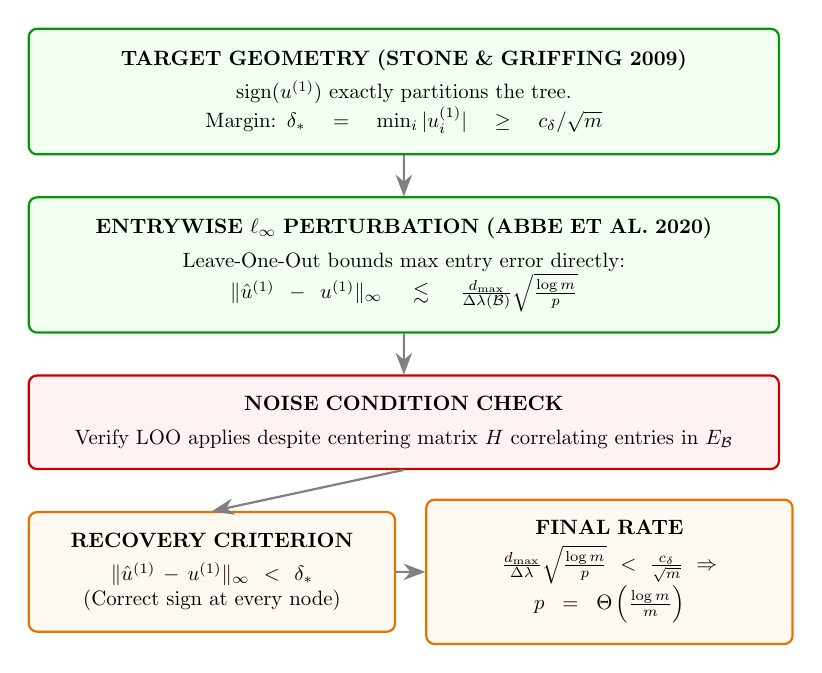
\begin{tikzpicture}[
        scale=0.75, transform shape,
        node distance=0.7cm and 0.5cm,
        box/.style={rectangle, draw, rounded corners=3pt, thick, align=center, inner sep=10pt, text width=12cm},
        boxhalf/.style={rectangle, draw, rounded corners=3pt, thick, align=center, inner sep=10pt, text width=5.5cm},
        cite/.style={draw=green!60!black, fill=green!5},
        prove/.style={draw=red!80!black, fill=red!5},
        deduce/.style={draw=orange!90!black, fill=orange!5},
        arrow/.style={-{Stealth[scale=1.2]}, thick, draw=gray}
    ]
    
    % Nodes
    \node (target) [box, cite] {\textbf{TARGET GEOMETRY (STONE \& GRIFFING 2009)} \\ \vspace{0.15cm} $\text{sign}(u^{(1)})$ exactly partitions the tree. \\ Margin: $\delta_* = \min_i |u_i^{(1)}| \ge c_\delta / \sqrt{m}$};
    
    \node (perturb) [box, cite, below=of target] {\textbf{ENTRYWISE $\ell_\infty$ PERTURBATION (ABBE ET AL. 2020)} \\ \vspace{0.15cm} Leave-One-Out bounds max entry error directly: \\ $\|\hat{u}^{(1)} - u^{(1)}\|_\infty \lesssim \frac{d_{\max}}{\Delta\lambda(\mathcal{B})} \sqrt{\frac{\log m}{p}}$};
    
    \node (noise) [box, prove, below=of perturb] {\textbf{NOISE CONDITION CHECK} \\ \vspace{0.15cm} Verify LOO applies despite centering matrix $H$ correlating entries in $E_{\mathcal{B}}$};
    
    \node (recovery) [boxhalf, deduce, below=of noise, xshift=-3.25cm] {\textbf{RECOVERY CRITERION} \\ \vspace{0.15cm} $\|\hat{u}^{(1)} - u^{(1)}\|_\infty < \delta_*$ \\ (Correct sign at every node)};
    
    \node (rate) [boxhalf, deduce, right=0.5cm of recovery] {\textbf{FINAL RATE} \\ \vspace{0.15cm} $\frac{d_{\max}}{\Delta\lambda} \sqrt{\frac{\log m}{p}} < \frac{c_\delta}{\sqrt{m}} \Rightarrow p = \Theta\left(\frac{\log m}{m}\right)$};
    
    % Arrows
    \draw [arrow] (target) -- (perturb);
    \draw [arrow] (perturb) -- (noise);
    \draw [arrow] (noise.south) -- (recovery.north);
    \draw [arrow] (recovery.east) -- (rate.west);
    
    \end{tikzpicture}
    \caption{The Leave-One-Out (LOO) proof route for single-stage exact recovery.}
    \label{fig:loo_route}
\end{figure}

\subsection{Full Entrywise Proof}

\begin{theorem}[Single-Stage Exact Recovery]
\label{thm:recovery}
Assume the spectral gap $\Delta\lambda = |\lambda_1(\mathcal{B})| - |\lambda_2(\mathcal{B})|$ is strictly positive. If the sampling rate satisfies
\begin{equation}
p = \Theta\left(\frac{d_{\max}^2}{\Delta\lambda^2 \cdot \delta_*^2} \log m\right)
\end{equation}
then with high probability $\text{sign}(\hat{u}^{(1)}) = \text{sign}(u^{(1)})$. For a tree with $\Delta\lambda \asymp m$ and $\delta_* \asymp 1/\sqrt{m}$ this is $p = \Theta(\frac{\log m}{m})$.
\end{theorem}

\begin{proof}
We bound the largest entry of the eigenvector error. The tool is the leave-one-out (LOO) bound, and the part of it we use is \cite{abbe2020entrywise}:

\begin{theorem}[Abbe et al. 2020, Theorem 2.1 (Consequence for Symmetric Matrices)]
Let $N$ be a symmetric matrix with eigendecomposition $N = U \Lambda U^\top$, and let $\hat{N} = N + E$ where $E$ is a symmetric noise matrix with independent mean-zero entries (up to symmetry). Let $\hat{U}$ denote the empirical top $r$ eigenvectors. Provided the spectral gap $\Delta\lambda$ is sufficiently large, there exists an orthogonal alignment matrix $W$ such that:
\begin{equation}
\|\hat{U} W - U\|_\infty \lesssim \frac{\|E U\|_\infty}{\Delta\lambda} + \frac{\|E\|_2 \|E\|_{\text{row\_max}}}{\Delta\lambda^2} \|U\|_\infty
\end{equation}
\end{theorem}

Here we use it with $r=1$: $U$ is the single vector $u^{(1)}$, $W$ is a sign flip, which we fix by taking the signs to be aligned, $N$ is $\mathcal{B}$, and $E$ is the centered noise $E_{\mathcal{B}}$. The matrix $\mathcal{B}$ is full rank, but only the gap $\Delta\lambda$ at the top of its spectrum enters the LOO expansion, which gives
\begin{equation}
\|\hat{u}^{(1)} - u^{(1)}\|_\infty \lesssim \frac{\|E_{\mathcal{B}} u^{(1)}\|_\infty}{\Delta\lambda} + \frac{\|E_{\mathcal{B}}\|_2 \|E_{\mathcal{B}}\|_{\text{row\_max}}}{\Delta\lambda^2} \|u^{(1)}\|_\infty
\end{equation}

We now bound each norm on the right for the centered noise matrix $E_{\mathcal{B}} = H E_{\mathcal{D}} H$.

\textbf{1. Bounding the first-order term $\|E_{\mathcal{B}} u^{(1)}\|_\infty$:} \\
Since the population vector is centered ($H u^{(1)} = u^{(1)}$), we have $E_{\mathcal{B}} u^{(1)} = H E_{\mathcal{D}} u^{(1)}$. The $i$-th entry of $E_{\mathcal{D}} u^{(1)}$ is:
\begin{equation}
(E_{\mathcal{D}} u^{(1)})_i = \sum_{j=1}^m (E_{\mathcal{D}})_{ij} u^{(1)}_j
\end{equation}
Because the entries $(E_{\mathcal{D}})_{ij}$ are independent with mean zero, and $u^{(1)}$ is a fixed vector, this is a sum of independent random variables. The variance of the sum is bounded by $\sum_j \frac{d_{\max}^2}{p} (u^{(1)}_j)^2 = \frac{d_{\max}^2}{p}$. The maximum absolute value of a single summand is bounded by $\frac{d_{\max}}{p} \|u^{(1)}\|_\infty$. By Bernstein's inequality, with high probability:
\begin{equation}
\|E_{\mathcal{D}} u^{(1)}\|_\infty \lesssim d_{\max} \sqrt{\frac{\log m}{p}}
\end{equation}
The centering matrix $H$ only subtracts the mean $\frac{1}{m}\mathbf{1}^\top E_{\mathcal{D}} u^{(1)}$, which is an average of these concentrated sums and is therefore of even smaller order. Thus, $\|E_{\mathcal{B}} u^{(1)}\|_\infty \lesssim d_{\max} \sqrt{\frac{\log m}{p}}$.

\textbf{2. Bounding the operator and row norms ($\|E_{\mathcal{B}}\|_2$ and $\|E_{\mathcal{B}}\|_{\text{row\_max}}$):} \\
By standard Matrix Bernstein inequalities \cite{tropp2012}, the operator norm of the independent noise matrix concentrates as $\|E_{\mathcal{D}}\|_2 \lesssim d_{\max} \sqrt{\frac{m}{p}}$. Because $H$ is a projector, $\|E_{\mathcal{B}}\|_2 \le \|E_{\mathcal{D}}\|_2 \lesssim d_{\max} \sqrt{\frac{m}{p}}$. 
Similarly, the row norm $\|e_i^\top E_{\mathcal{B}}\|_2$ is dominated by the Euclidean norm of a row of $E_{\mathcal{D}}$, which is the square root of $m$ independent variables each with variance $d_{\max}^2/p$. By scalar concentration, $\|E_{\mathcal{B}}\|_{\text{row\_max}} \lesssim d_{\max} \sqrt{\frac{m}{p}}$.

\textbf{3. Synthesis and Recovery Criterion:} \\
Putting the three bounds of steps 1 and 2 into the LOO bound leaves two terms:
\begin{equation}
\label{eq:two-terms}
\|\hat{u}^{(1)} - u^{(1)}\|_\infty \;\lesssim\;
\underbrace{\frac{d_{\max}}{\Delta\lambda} \sqrt{\frac{\log m}{p}}}_{\text{(I) linear in the noise}}
\;+\;
\underbrace{\frac{d_{\max}^2 m}{p \, \Delta\lambda^2} \, \|u^{(1)}\|_\infty}_{\text{(II) quadratic in the noise}}
\end{equation}
The two are of different kinds. Term (I) is the noise acting once, along the population
vector: it comes from $\|E_{\mathcal{B}} u^{(1)}\|_\infty$, one Bernstein sum per
coordinate. Term (II) is the noise acting twice, through the product
$\|E_{\mathcal{B}}\|_2 \|E_{\mathcal{B}}\|_{\text{row\_max}}$, which is why it carries
$\Delta\lambda^{-2}$ and a second factor of $d_{\max}$.

A sign is read correctly at every leaf as soon as the total deviation stays below the
margin, so we ask each term to be smaller than $\delta_*/2$. With the delocalization of
\Cref{sec:target}, $\|u^{(1)}\|_\infty \asymp 1/\sqrt{m}$ and $\delta_* \asymp
1/\sqrt{m}$, this asks
\begin{align}
\text{(I)} &: \quad \frac{d_{\max}}{\Delta\lambda} \sqrt{\frac{\log m}{p}}
   \;<\; \frac{c_\delta}{2\sqrt{m}}
   &&\Longrightarrow\quad p \;\gtrsim\; \frac{d_{\max}^2 \, m \log m}{\Delta\lambda^2},
   \label{eq:cond-linear} \\[2pt]
\text{(II)} &: \quad \frac{d_{\max}^2 m}{p \, \Delta\lambda^2 \sqrt{m}}
   \;<\; \frac{c_\delta}{2\sqrt{m}}
   &&\Longrightarrow\quad p \;\gtrsim\; \frac{d_{\max}^2 \, m}{\Delta\lambda^2}.
   \label{eq:cond-quadratic}
\end{align}
The two requirements differ by exactly the factor $\log m$, so \eqref{eq:cond-linear} is
the binding one and \eqref{eq:cond-quadratic} is satisfied automatically at that rate.
Hence
\begin{equation}
p \;=\; \Theta\!\left( \frac{d_{\max}^2 \, m \log m}{\Delta\lambda^2} \right)
\end{equation}
is enough for $\mathrm{sign}(\hat{u}^{(1)}) = \mathrm{sign}(u^{(1)})$ at every leaf, and
with $\Delta\lambda \asymp m$ this is the $p = \Theta(\log m / m)$ of the statement.
\end{proof}

\subsection{Open Question: How Do $\Delta\lambda$ and $\delta_*$ Depend on the Tree?}
\label{sec:open}

The rate above is written in terms of two numbers, and both can be derived once the tree is
fixed:
\begin{itemize}
\item the gap $\Delta\lambda = |\lambda_1(\mathcal{B})| - |\lambda_2(\mathcal{B})|$, which
says how far the leading direction of $\mathcal{B}$ stands out from the next one;
\item the smallest entry $\delta_* = \min_i |u^{(1)}_i|$, which says how close the closest
leaf comes to sitting on the fence between the two sides.
\end{itemize}
We put $\Delta\lambda \asymp m$ and $\delta_* \asymp 1/\sqrt{m}$ into the general rate to
get $p \gtrsim \log m / m$. What is open is how to read those two numbers off a tree:

\begin{quote}
Given a weighted tree $T$ with $m$ leaves, how small can $\Delta\lambda$ and $\delta_*$
be, in terms of the shape of $T$ and the lengths of its branches?
\end{quote}

\Cref{cor:two-numbers} already puts the question in a more familiar form. Since
$\Delta\lambda/|\lambda_1| = 1 - \mu_1/\mu_2$ and $\delta_* = \min_i |y_i|$, what is wanted
is a lower bound on the algebraic connectivity $\mu_1$ of the reduced graph $G_D$, a bound
on the ratio $\mu_1/\mu_2$, and a lower bound on the smallest entry of its Fiedler vector
--- three questions about one weighted graph built from the tree. \Cref{sec:vs-laplacian}
is the other way in: it reaches the same two numbers from the similarity Laplacian, at the
price of the row-sum spread and a term of the order of the squared distances. What each kind of tree
does to them is collected in Appendix~\ref{app:answer}.

\section{The Connection Between $S$ and $\mathcal{D}$}
\label{sec:vs-laplacian}

The other way to cut a tree from the same data is to turn distances into similarities and
take the Fiedler vector of the similarity Laplacian $L_S$ \cite{fiedler1975property}.

Write $S = e^{-\mathcal{D}}$ entrywise, with $S_{ii} = 1$, and
$L_S = \mathrm{Deg}(S) - S$.

By Taylor expansion of $e^{-t}$ around $t=0$,
\begin{equation}
\label{eq:taylor}
S \;=\; J - \mathcal{D} + \Gamma, \qquad
\Gamma_{ij} := e^{-\mathcal{D}_{ij}} - 1 + \mathcal{D}_{ij}, \qquad
0 \le \Gamma_{ij} \le \tfrac{1}{2}\mathcal{D}_{ij}^2 ,
\end{equation}
with $J$ the all-ones matrix. Applying $W \mapsto \mathrm{Deg}(W) - W$ term by term,
\begin{equation}
\label{eq:LS-in-D}
L_S \;=\; (mI - J) \;-\; \big(\mathrm{Deg}(\mathcal{D}) - \mathcal{D}\big)
\;+\; \big(\mathrm{Deg}(\Gamma) - \Gamma\big) .
\end{equation}
Centering brings in the distance operator. With
$\mathrm{Deg}(\mathcal{D}) = \mathrm{diag}(d)$, $d_i = \sum_j \mathcal{D}_{ij}$, and
$\bar{d}$ the mean of the $d_i$, and using $HJH = 0$ and $H\mathcal{D}H = \mathcal{B}$,
\begin{equation}
\label{eq:conjugated}
H L_S H \;=\; (m - \bar{d})\,H \;+\; \mathcal{B}
\;-\; H \mathrm{diag}(d - \bar{d}) H
\;+\; H\big(\mathrm{Deg}(\Gamma) - \Gamma\big)H ,
\end{equation}
with no approximation so far.

\begin{lemma}[When the two routes share an eigenvector]
\label{lem:bridge}
If $d_i = \bar{d}$ for every leaf and $\Gamma = 0$, then
$H L_S H = (m - \bar{d})H + \mathcal{B}$, and the Fiedler vector of $L_S$ is $u^{(1)}$.
\end{lemma}

\begin{proof}
The last two terms of \eqref{eq:conjugated} vanish, so on the centered subspace the two
operators differ by a multiple of the identity. Their eigenvectors coincide, and the
smallest eigenvalue of $L_S$ there belongs to the most negative eigenvalue of
$\mathcal{B}$.
\end{proof}

So the two routes are separated by the row-sum spread $\max_i|d_i - \bar{d}|$ and by
$\Gamma$, which is second order in the distances;
Appendix~\ref{app:operators} reports how far apart the two vectors sit in practice.

\newpage
\bibliographystyle{plain}
\bibliography{bibi}

\newpage
\appendix

\section{Answering the Open Question by Simulation}
\label{app:operators}

% [Reviewer Note: every number below is read from the caches in
% analysis/notebooks_cache/eta_by_operator/ --- {kingman,bd}_n1000_L10000.npz (splits),
% spectra_sample_n1000_L10000_R200.npz, vectors_sample_n1000_L10000_R200.npz --- and the
% figures are produced by the final cell of analysis/supporting/eta_by_operator.ipynb.]

Jukes--Cantor sequences of length $L = 10^4$ on trees with $m = 1000$ leaves, in two pools:
Kingman coalescent and pure birth (rate $0.5$, no extinction). Split statistics use $1000$
trees per model, spectra and vectors $200$, the route comparison $15$. Entries are medians,
with the quartile range in parentheses.

\begin{table}[H]
\centering
\begin{tabular}{@{}lrrcrc@{}}
\toprule
& \multicolumn{3}{c}{$\mathcal{B} = H\mathcal{D}H$} & \multicolumn{2}{c}{$L_S$} \\
\cmidrule(lr){2-4}\cmidrule(lr){5-6}
Model & $|\lambda_1|$ & $|\lambda_2|$ & $(|\lambda_1|-|\lambda_2|)/|\lambda_1|$
      & $\lambda_2$ & $(\lambda_3-\lambda_2)/\lambda_3$ \\
\midrule
Kingman      & $352.1$  & $114.9$ & $0.60$ $(0.44,\,0.80)$ & $244.2$   & $0.20$ $(0.08,\,0.40)$ \\
birth--death & $1200.8$ & $721.1$ & $0.38$ $(0.27,\,0.47)$ & $0.0260$  & $0.25$ $(0.11,\,0.44)$ \\
\bottomrule
\end{tabular}
\caption{Leading spectrum of each operator, $200$ trees per model. $\mathcal{B}$ is
negative semi-definite, so its eigenvalues are ordered by magnitude; $L_S$ is ordered
ascending, and $\lambda_1(L_S) = 0$.}
\label{tab:app-spectrum}
\end{table}

\begin{table}[H]
\centering
\begin{tabular}{@{}lccc@{}}
\toprule
Model & $\sqrt{m}\,\delta_*$ & $\sqrt{m}\,\|u^{(1)}\|_\infty$ & $\sqrt{m}\,\|v^{(2)}\|_\infty$ \\
\midrule
Kingman      & $0.356$  $(0.068,\,0.659)$   & $1.59$ & $1.9$ \\
birth--death & $0.0241$ $(0.00038,\,0.308)$ & $1.80$ & $2.0$ \\
\bottomrule
\end{tabular}
\caption{Entries of the classifying vectors, $200$ trees per model, each vector normalised
to unit length and scaled by $\sqrt{m}$; the range in parentheses is the $10$th to $90$th
percentile. $\delta_* = \min_i |u^{(1)}_i|$ and $v^{(2)}$ is the Fiedler vector of $L_S$.}
\label{tab:app-vectors}
\end{table}

\begin{table}[H]
\centering
\begin{tabular}{@{}lccccccc@{}}
\toprule
& \multicolumn{2}{c}{valid edge (\%)} & \multicolumn{2}{c}{median $\eta$} & & & \\
\cmidrule(lr){2-3}\cmidrule(lr){4-5}
Model & $\mathcal{B}$ & $L_S$ & $\mathcal{B}$ & $L_S$ & same split (\%)
      & $|\langle u^{(1)}, v^{(2)}\rangle|$ & $\max_i|d_i-\bar d|/\bar d$ \\
\midrule
Kingman      & $98.6$ & $99.6$ & $1.85$ & $3.00$ & $64$ & $0.98$ & $0.49$ \\
birth--death & $55.5$ & $99.6$ & $1.53$ & $3.08$ & $33$ & $0.97$ & $0.17$ \\
\bottomrule
\end{tabular}
\caption{Which split each operator reads, $1000$ trees per model; the last two columns are
over $15$ trees per model. A split is a valid edge when it is a single-edge bipartition of
the true tree, and $\eta$ is the ratio of the two clan sizes.}
\label{tab:app-splits}
\end{table}

Each panel of the figures below carries its own scale: the four matrices are on separate
colour scales, the eigenvalue histograms clip the $\lambda_1(L_S) \equiv 0$ bar, and the
entry histograms use logarithmic counts with dotted lines at $\pm 1$.

\begin{figure}[H]
    \centering
    \begin{subfigure}[t]{0.46\textwidth}
        \captionsetup{singlelinecheck=false, justification=raggedright, skip=1pt}
        \subcaption{$v^{(2)}$ of $L_S$}
        
\includegraphics[width=\textwidth]{figures/dr2_tree_vec_S.png}
        \label{fig:app-tree-a}
    \end{subfigure}
    \hfill
    \begin{subfigure}[t]{0.46\textwidth}
        \captionsetup{singlelinecheck=false, justification=raggedright, skip=1pt}
        \subcaption{$u^{(1)}$ of $\mathcal{B}=H\mathcal{D}H$}
        
\includegraphics[width=\textwidth]{figures/dr2_tree_vec_B.png}
        \label{fig:app-tree-b}
    \end{subfigure}
    \caption{One Kingman tree, cut by each vector; the pool's maximum-disagreement tree,
    split $505/495$ by $u^{(1)}$ and $998/2$ by $v^{(2)}$.}
    \label{fig:app-tree}
\end{figure}

\begin{figure}[H]
    \centering
    \begin{subfigure}[t]{0.24\textwidth}
        \captionsetup{singlelinecheck=false, justification=raggedright, skip=1pt}
        \subcaption{$S=e^{-\mathcal{D}}$}
        
\includegraphics[width=\textwidth]{figures/dr2_mat_S.png}
    \end{subfigure}
    \hfill
    \begin{subfigure}[t]{0.24\textwidth}
        \captionsetup{singlelinecheck=false, justification=raggedright, skip=1pt}
        \subcaption{$L_S=\mathrm{Deg}(S)-S$}
        
\includegraphics[width=\textwidth]{figures/dr2_mat_L.png}
    \end{subfigure}
    \hfill
    \begin{subfigure}[t]{0.24\textwidth}
        \captionsetup{singlelinecheck=false, justification=raggedright, skip=1pt}
        \subcaption{$\mathcal{D}=-\log S$}
        
\includegraphics[width=\textwidth]{figures/dr2_mat_D.png}
    \end{subfigure}
    \hfill
    \begin{subfigure}[t]{0.24\textwidth}
        \captionsetup{singlelinecheck=false, justification=raggedright, skip=1pt}
        \subcaption{$\mathcal{B}=H\mathcal{D}H$}
        
\includegraphics[width=\textwidth]{figures/dr2_mat_B.png}
    \end{subfigure}
    \caption{The four matrices on the tree of \Cref{fig:app-tree}, leaves in clade order;
    the degree diagonal of $L_S$ is masked.}
    \label{fig:app-mat}
\end{figure}

\begin{figure}[H]
    \centering
    \begin{subfigure}[t]{0.42\textwidth}
        \captionsetup{singlelinecheck=false, justification=raggedright, skip=1pt}
        \subcaption{Kingman, $L_S$}
        
\includegraphics[width=\textwidth]{figures/dr2_eig_kingman_L.png}
    \end{subfigure}
    \hfill
    \begin{subfigure}[t]{0.42\textwidth}
        \captionsetup{singlelinecheck=false, justification=raggedright, skip=1pt}
        \subcaption{Kingman, $\mathcal{B}$}
        
\includegraphics[width=\textwidth]{figures/dr2_eig_kingman_B.png}
    \end{subfigure}

    \begin{subfigure}[t]{0.42\textwidth}
        \captionsetup{singlelinecheck=false, justification=raggedright, skip=1pt}
        \subcaption{birth--death, $L_S$}
        
\includegraphics[width=\textwidth]{figures/dr2_eig_bd_L.png}
    \end{subfigure}
    \hfill
    \begin{subfigure}[t]{0.42\textwidth}
        \captionsetup{singlelinecheck=false, justification=raggedright, skip=1pt}
        \subcaption{birth--death, $\mathcal{B}$}
        
\includegraphics[width=\textwidth]{figures/dr2_eig_bd_B.png}
    \end{subfigure}
    \caption{First two eigenvalues per model and route, $200$ trees each: grey
    $\lambda_1$, coloured $\lambda_2$, dashed at the medians (\Cref{tab:app-spectrum}).}
    \label{fig:app-eig}
\end{figure}

\begin{figure}[H]
    \centering
    \begin{subfigure}[t]{0.42\textwidth}
        \captionsetup{singlelinecheck=false, justification=raggedright, skip=1pt}
        \subcaption{Kingman, Fiedler of $L_S$}
        
\includegraphics[width=\textwidth]{figures/dr2_vec_kingman_L.png}
    \end{subfigure}
    \hfill
    \begin{subfigure}[t]{0.42\textwidth}
        \captionsetup{singlelinecheck=false, justification=raggedright, skip=1pt}
        \subcaption{Kingman, $u^{(1)}$}
        
\includegraphics[width=\textwidth]{figures/dr2_vec_kingman_B.png}
    \end{subfigure}

    \begin{subfigure}[t]{0.42\textwidth}
        \captionsetup{singlelinecheck=false, justification=raggedright, skip=1pt}
        \subcaption{birth--death, Fiedler of $L_S$}
        
\includegraphics[width=\textwidth]{figures/dr2_vec_bd_L.png}
    \end{subfigure}
    \hfill
    \begin{subfigure}[t]{0.42\textwidth}
        \captionsetup{singlelinecheck=false, justification=raggedright, skip=1pt}
        \subcaption{birth--death, $u^{(1)}$}
        
\includegraphics[width=\textwidth]{figures/dr2_vec_bd_B.png}
    \end{subfigure}
    \caption{Pooled entries of the classifying vectors, $\sqrt{m}$-scaled and oriented
    minority-positive; pool maxima $5.7$ for $u^{(1)}$ and $16.4$ ($21.1$) for $v^{(2)}$ on
    Kingman (birth--death) trees, against $\sqrt{m} = 31.6$ (\Cref{tab:app-vectors}).}
    \label{fig:app-vec}
\end{figure}


\paragraph{Bottom line.} The upper half of \Cref{as:deloc} holds on both models
($\sqrt{m}\|u^{(1)}\|_\infty \approx 1.6$ and $1.8$), the lower half holds on Kingman trees
with a small constant ($\sqrt{m}\,\delta_* = 0.36$) and fails on pure-birth trees
($0.024$, with a tenth of them below $0.0004$).

\begin{landscape}
\section{Answering the Open Question by Theory}
\label{app:answer}

\begin{table}[H]
\centering
\begin{tabular}{@{}p{3.4cm}p{3.6cm}p{3.4cm}p{10.5cm}@{}}
\toprule
Tree & $\delta_* \approx$ & $\Delta\lambda \approx$ & Note \\
\midrule
Balanced binary
  & $1/\sqrt{m}$
  & order $m$
  & Symmetry fixes the vector: $u^{(1)}$ is two-valued with $\alpha = 1/2$, so every entry
    has the same size and the margin is as large as it can be. \\[6pt]
Kingman coalescent
  & $\sqrt{\alpha/(1-\alpha)}\,/\sqrt{m}$
  & a constant fraction of $|\lambda_1|$
  & Theory. The topology is Yule, whose root split is uniform in size
    \cite{steel2001yule,aldous2001stochastic}, so the smaller side is
    $\alpha \sim \mathrm{U}\{1/m,\dots,1/2\}$: typically of order one, with a tail down to
    $1/m$ when the split peels off a single leaf. The last coalescence lasts
    $\mathrm{Exp}(1)$ against a tree height of mean $2(1-1/m)$
    \cite{kingman1982coalescent,wakeley2009coalescent}, so the deepest split stands clear
    of the next one by a fixed share of $|\lambda_1|$ rather than a vanishing one.
    Measured values in \Cref{tab:app-spectrum,tab:app-vectors}. \\[6pt]
Pure birth (Yule branch lengths)
  & $0.024/\sqrt{m}$
  & $0.38\,|\lambda_1|$
  & Measured, $200$ trees at $m = 1000$ (\Cref{tab:app-spectrum,tab:app-vectors}). The
    topology law is the same as the row above, so $\alpha$ is drawn from the same
    distribution; what changes is where the branch lengths sit, and that alone moves the
    median margin down by a factor of $15$ against the coalescent's $0.36/\sqrt{m}$. \\[6pt]
Caterpillar, very uneven branch lengths (extreme)
  & well below $1/\sqrt{m}$
  & well below $m$
  & The leading vector puts most of its weight on a handful of leaves, which is
    $\alpha \to 1/m$ in \eqref{eq:two-block-margin}, and the remaining entries are what
    sets $\delta_*$. How far below $1/\sqrt{m}$ the margin goes, and how far below $m$ the
    gap goes, is the open part of the question. \\
\bottomrule
\end{tabular}
\caption{What each kind of tree does to the two numbers the rate is written in.}
\label{tab:tree-kinds}
\end{table}

Reference point for the $\delta_*$ column: a two-valued $u^{(1)}$ that puts a fraction
$\alpha \le 1/2$ of the leaves on the smaller side has
\begin{equation}
\label{eq:two-block-margin}
\delta_* \;=\; \frac{1}{\sqrt{m}}\sqrt{\frac{\alpha}{1-\alpha}} .
\end{equation}
\end{landscape}

\end{document}
